\section{Resultados e Discussão}

% =============================================================================
\subsection{MVP1: Análise Exploratória}

A matriz de correlação (Figura~\ref{fig:matriz_corr}) mostra blocos de atributos
fortemente correlacionados entre si, em especial as taxas de erro de conexão e as
contagens por \en{host} de destino. Os atributos mais correlacionados com o rótulo
de ataque são as taxas de erro SYN --- \cod{dst\_host\_srv\_serror\_rate} (0,655),
\cod{dst\_host\_serror\_rate} (0,652), \cod{serror\_rate} (0,651) e
\cod{srv\_serror\_rate} (0,648) --- seguidas de \cod{count} (0,576). São
exatamente os sinais de inundação SYN, como o \en{neptune}, que responde por 70\% dos
ataques do treino.

\begin{figure}[H]
  \centering
  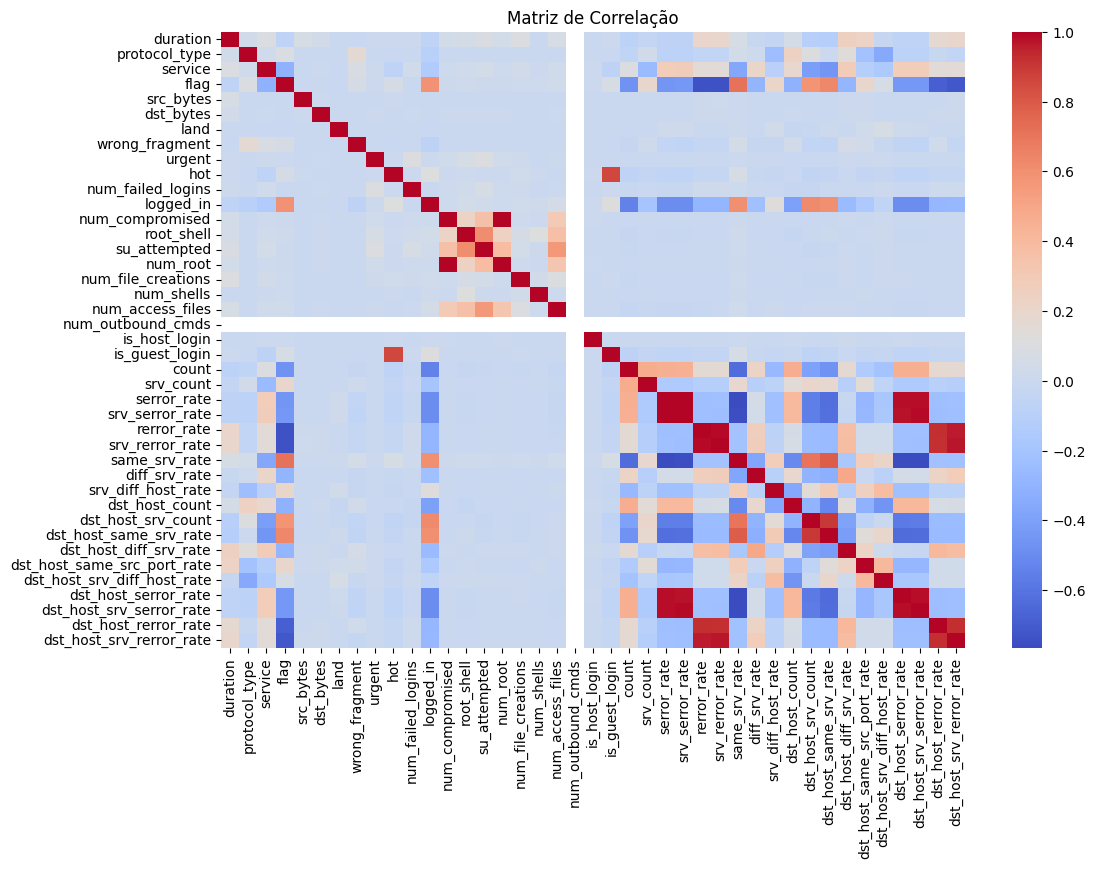
\includegraphics[width=0.95\columnwidth]{matriz_corr.png}
  \caption{Matriz de correlação de \en{Pearson} dos atributos numéricos do NSL-KDD.}
  \label{fig:matriz_corr}
\end{figure}

O PCA precisou de 22 dos 36 componentes para reter 95,43\% da variância
(Figura~\ref{fig:pca_variancia}). A projeção nos dois primeiros componentes
(Figura~\ref{fig:pca_classes}) mostra que DoS e \en{Probe} ocupam regiões
distintas do tráfego normal, enquanto R2L e U2R se sobrepõem a ele --- coerente
com a natureza desses ataques, que se parecem com sessões legítimas no nível de
conexão.

\begin{figure}[H]
  \centering
  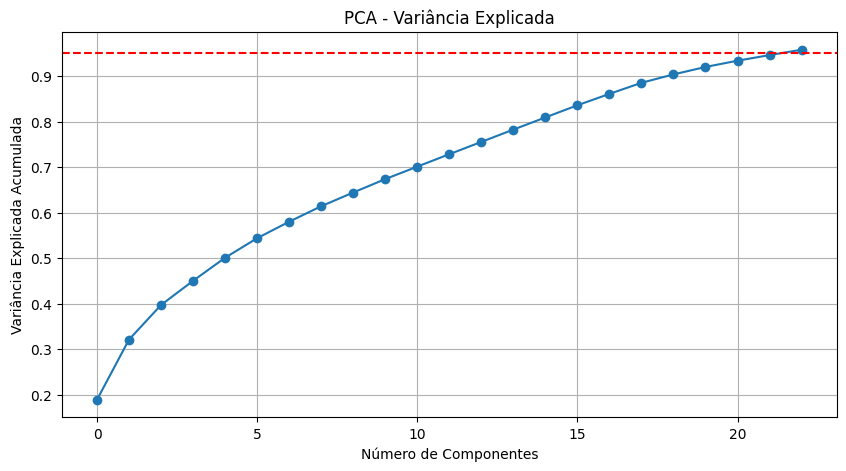
\includegraphics[width=\columnwidth,height=5cm]{pcaXvariancia.png}
  \caption{Variância explicada acumulada em função do número de componentes do PCA.}
  \label{fig:pca_variancia}
\end{figure}

\begin{figure}[H]
  \centering
  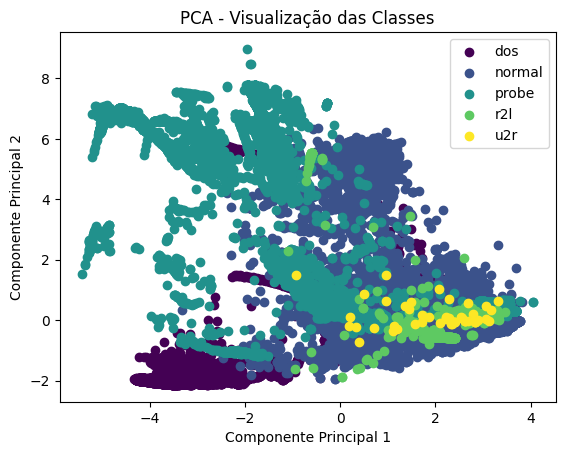
\includegraphics[width=0.95\columnwidth]{pca_classes.png}
  \caption{Projeção nos dois primeiros componentes principais, por categoria.}
  \label{fig:pca_classes}
\end{figure}

% =============================================================================
\subsection{MVP1: Comparação de Algoritmos}

A Tabela~\ref{tab:mvp1} resume a comparação na partição de validação. Os modelos
baseados em árvore dominam as métricas de classificação, mas o custo
computacional separa os candidatos. O \en{Random Forest} tem o maior
\en{F1-score} (0,9984), porém treina em 6,7~s e prediz em 0,20~s. A
\en{Decision Tree} fica a 0,0007 de distância no \en{F1-score}, treina 9 vezes mais
rápido e prediz 56 vezes mais rápido (3,5~ms para cerca de 25 mil registros). O KNN
não tem custo de treino, mas leva 16~s para predizer, inviável em fluxo contínuo,
e o SVM com \en{kernel} linear em lote foi o mais lento em ambas as fases (198~s de
treino). Pelo equilíbrio entre acurácia e latência, a \en{Decision Tree} foi
selecionada no MVP1.

\begin{table}[H]
\centering
\footnotesize
\setlength{\tabcolsep}{2.5pt}
\begin{tabular}{l c c c c r r}
\toprule
\textbf{Modelo} & \textbf{Acc} & \textbf{Prec} & \textbf{Rec} & \textbf{F1} & \textbf{Treino (s)} & \textbf{Teste (s)} \\
\midrule
RF  & 0,9985 & 0,9991 & 0,9977 & 0,9984 &   6,70 &  0,196 \\
DT  & 0,9978 & 0,9977 & 0,9976 & 0,9977 &   0,72 &  0,004 \\
KNN & 0,9919 & 0,9900 & 0,9926 & 0,9913 &   0,00 & 16,014 \\
LR  & 0,9488 & 0,9576 & 0,9312 & 0,9442 &   1,89 &  0,002 \\
SVM & 0,9532 & 0,9658 & 0,9325 & 0,9489 & 198,34 &  7,605 \\
\bottomrule
\end{tabular}
\caption{Desempenho na validação (20\% estratificado do \cod{KDDTrain+}, 36 atributos padronizados).}
\label{tab:mvp1}
\end{table}

A seleção por importância mostrou que o sinal está concentrado em poucos
atributos: \cod{src\_bytes} sozinho responde por 74,9\% da importância da árvore,
os dois primeiros por 80\% e os cinco primeiros por 90\%
(Figura~\ref{fig:importancia}). Variando o número de atributos de 5 a 38
(Figura~\ref{fig:n_features}), a acurácia já é 0,9961 com 5 atributos e atinge o
máximo de 0,9980 com 17, com variação inferior a 0,0005 a partir daí. Os
17 atributos selecionados são, em ordem: \cod{src\_bytes},
\cod{dst\_host\_srv\_count}, \cod{count}, \cod{dst\_bytes},
\cod{dst\_host\_same\_src\_port\_rate}, \cod{num\_compromised},
\cod{dst\_host\_same\_srv\_rate}, \cod{srv\_count}, \cod{diff\_srv\_rate},
\cod{duration}, \cod{dst\_host\_count}, \cod{dst\_host\_rerror\_rate},
\cod{wrong\_fragment}, \cod{dst\_host\_diff\_srv\_rate},
\cod{dst\_host\_srv\_serror\_rate}, \cod{is\_guest\_login} e
\cod{dst\_host\_serror\_rate}. O resultado está em linha com a literatura, que
relata conjuntos de 9 a 20 atributos sem perda de desempenho
\cite{Thakkar2021Survey, Othman2018Intrusion, Rathore2016RealTime}.

\begin{figure}[H]
  \centering
  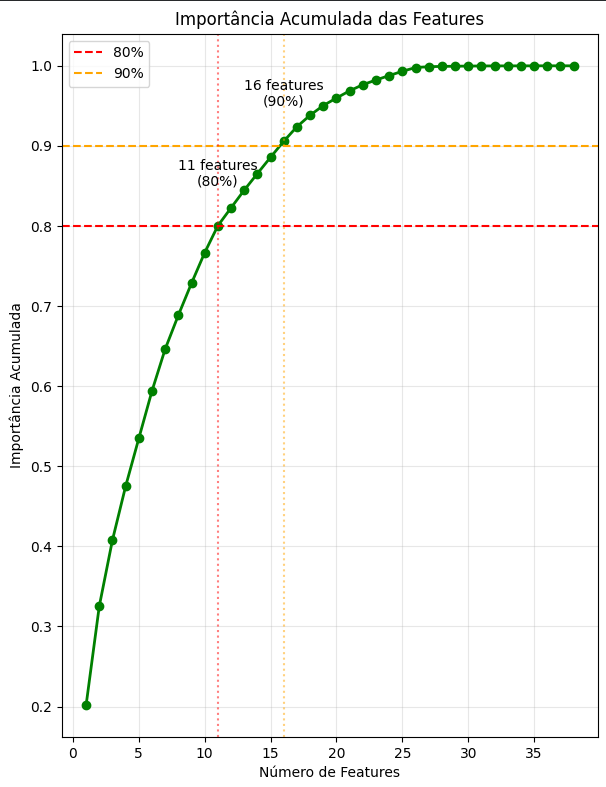
\includegraphics[width=\columnwidth,height=7.5cm]{Importancia_features.png}
  \caption{Importância dos atributos segundo a \en{Decision Tree}.}
  \label{fig:importancia}
\end{figure}

\begin{figure}[H]
  \centering
  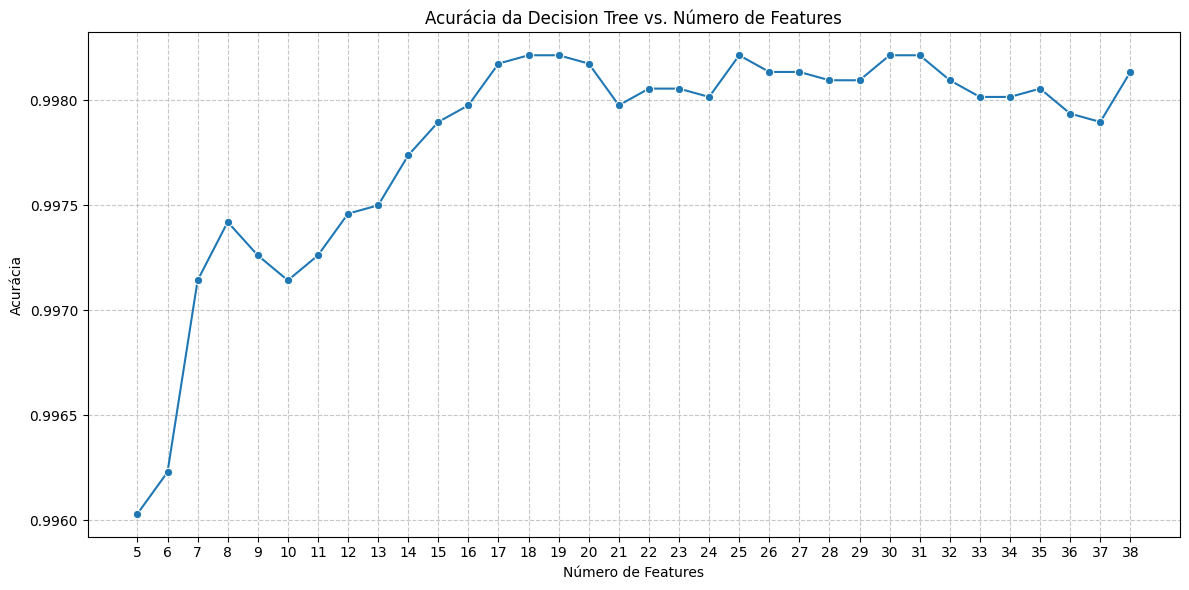
\includegraphics[width=\columnwidth,height=5cm]{decisiontree_features.png}
  \caption{Acurácia da \en{Decision Tree} em função do número de atributos mais importantes.}
  \label{fig:n_features}
\end{figure}

% =============================================================================
\subsection{MVP1: Generalização para Ataques Novos}

Retreinado sobre todo o \cod{KDDTrain+} e aplicado ao \cod{KDDTest+}, o melhor
modelo da validação (\en{Random Forest}) caiu para \textbf{77,92\% de acurácia} e
\textbf{63,22\% de \en{recall}}, mantendo precisão de 96,93\% (F1 = 0,7653). A
matriz de confusão (Figura~\ref{fig:confusao}) mostra que o erro é quase todo
falso negativo: 4.720 dos 12.833 ataques do teste foram classificados como
normais, contra apenas 257 falsos positivos.

\begin{figure}[H]
  \centering
  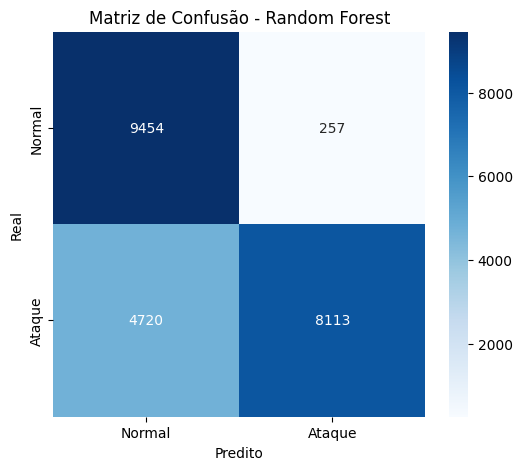
\includegraphics[width=0.75\columnwidth]{matriz_confusao_kddtest.png}
  \caption{Matriz de confusão do \en{Random Forest} no \cod{KDDTest+}.}
  \label{fig:confusao}
\end{figure}

Esse é o resultado mais importante do MVP1. A acurácia de 99,8\% mede a capacidade
de reconhecer ataques \emph{já vistos}; diante de tipos ausentes do treino, o
classificador supervisionado os trata como normais e falha em silêncio. O modelo
não “erra para o lado seguro”: quando não reconhece, declara benigno. A divisão
aleatória do próprio \cod{KDDTrain+}, prática comum na literatura, superestima
o desempenho real \cite{Sommer2010Outside}. Daí derivam três requisitos do MVP2:
(i) um detector não supervisionado, que não dependa de ter visto o ataque; (ii)
um classificador supervisionado alimentado continuamente por rótulos da própria
rede; e (iii) avaliação por cenário de ataque, e não por acurácia agregada.

% =============================================================================
\subsection{MVP2: Ponto Cego do Isolation Forest}

O Estágio 1 foi avaliado com o \en{golden set} real de FTP-Patator do CIC-IDS-2017:
3.958 fluxos de ataque contra 93.883 fluxos de fundo da mesma rede e horário,
com modelo treinado sobre 26.507 fluxos benignos da mesma captura. O resultado foi
\textbf{\en{recall} 0,00} contra o piso de 0,85 do cenário. O ROC-AUC de 0,781 e a
precisão média de 0,0887 (contra 0,0405 de base) indicam alguma separação, mas
para \emph{qualquer} nível de \en{recall} o custo é de 22\% de falso positivo: o
limiar que captura 50\% do ataque (0,4689) é praticamente o mesmo que captura 99\%
(0,4679), porque todos os fluxos de ataque recebem quase o mesmo escore.

O problema não está nos atributos. Contra a mediana benigna, o ataque tem duração
147 vezes maior, \cod{std\_iat} 68 vezes, \cod{mean\_iat} 13 vezes e
\cod{n\_packets} 7 vezes. A causa é estrutural: 3.958 fluxos quase idênticos formam
um aglomerado denso, e o \en{Isolation Forest} isola pontos \emph{raros}
(Equação~\ref{eq:if}). Quanto mais o atacante repete, mais normal ele fica. A
ordenação resultante é \emph{benigno atípico $>$ ataque $>$ benigno típico}, e
nenhum limiar separa as classes --- ajustar o \en{contamination} não resolve. É a
mesma família do beacon de 6~h: ataques cuja assinatura está na repetição ao longo
do tempo, e não no fluxo individual.

% =============================================================================
\subsection{MVP2: Estágio 2 Recupera os Ataques Densos}

Para validar a premissa do Estágio 2, um SVM linear foi treinado nos mesmos 17
atributos e avaliado em conjuntos de teste separados, cenário a cenário
(Tabela~\ref{tab:e2}). O classificador supervisionado recupera integralmente os
ataques densos que o \en{Isolation Forest} não vê, inclusive a força bruta.

\begin{table}[H]
\centering
\footnotesize
\begin{tabular}{l c c}
\toprule
\textbf{Cenário} & \textbf{\en{Isolation Forest}} & \textbf{SVM linear} \\
\midrule
recon            & 0,36  & 1,00  \\
beacon\_6h       & 0,08  & 1,00  \\
brute\_force     & 0,00  & 1,00  \\
\midrule
FPR (benigno)    & 0,001 & 0,000 \\
\bottomrule
\end{tabular}
\caption{\en{Recall} por cenário e taxa de falso positivo, mesmos atributos e dados.}
\label{tab:e2}
\end{table}

Esses valores devem ser lidos com cautela. São resultados \emph{em distribuição}:
o SVM foi testado sobre formas de ataque que viu rotuladas no treino. Como mostrou
o MVP1, um classificador supervisionado não generaliza para ataques novos --- que
continuam sendo responsabilidade do Estágio 1. Em produção, o rótulo vem do
analista, é ruidoso e é enviesado pelo que o Estágio 1 decidiu mostrar. A Tabela
não mede detecção geral; mede que os dois estágios são \emph{complementares}: o não
supervisionado pega o raro e o novo, o supervisionado pega o conhecido e o denso.

% =============================================================================
\subsection{MVP2: Contamination e Teto de Falso Positivo}

Em um \en{pool} majoritariamente limpo, a taxa de falso positivo do
\en{Isolation Forest} tende ao valor de \en{contamination}, que é literalmente a
fração que o modelo foi instruído a marcar. Medido no \en{golden set}: 0,03 $\to$
FPR 0,026; 0,01 $\to$ 0,006; 0,005 $\to$ 0,001. Consequentemente, se o teto de
falso positivo do portão for menor que o \en{contamination}, \emph{nenhum}
candidato passa, e o sintoma se parece com degradação do modelo quando é apenas
aritmética da configuração. A configuração inicial tinha exatamente esse defeito
(teto de 0,02 contra \en{contamination} de 0,03), e o comando de treino passou a
emitir um aviso nesse caso.

A faixa utilizável é estreita: com 0,03 o candidato reprova por falso positivo;
com 0,01 passa; com 0,005 reprova porque o \en{recall} de \cod{beacon\_1h} cai
para 0,04 e o de \cod{beacon\_6h} para 0,06, enquanto \cod{recon} permanece em
1,00. Beacon é anomalia sutil e precisa de limiar mais frouxo; varredura sobrevive
a qualquer limiar. Uma métrica agregada teria escondido essa diferença.

% =============================================================================
\subsection{MVP2: Explicação Não Mede Detecção}

Uma hipótese natural seria usar a fidelidade da árvore \en{surrogate} como
gatilho de retreino. A Tabela~\ref{tab:surrogate} mostra por que isso não
funciona: com o \en{pool} envenenado por 10\% de tráfego C2, a detecção dos beacons
foi a zero enquanto a fidelidade variou um décimo de ponto percentual.

\begin{table}[H]
\centering
\footnotesize
\setlength{\tabcolsep}{3pt}
\begin{tabular}{l c c c c}
\toprule
\textbf{Regime do \en{pool}} & \textbf{Fidelid.} & \textbf{F1} & \textbf{bcn1h} & \textbf{bcn6h} \\
\midrule
Limpo                   & 0,997 & 0,838 & 0,85 & 0,98 \\
Envenenado (10\% C2)    & 0,996 & 0,780 & \textbf{0,00} & \textbf{0,01} \\
Deriva legítima         & 0,997 & 0,827 & 0,70 & 0,92 \\
\bottomrule
\end{tabular}
\caption{Fidelidade da árvore \en{surrogate} contra \en{recall} real por cenário.}
\label{tab:surrogate}
\end{table}

Quando o C2 vira normal, a floresta deixa de marcá-lo e a árvore reproduz esse
silêncio com fidelidade perfeita: as duas concordam em estar erradas. Além disso,
a queda de F1 causada pelo envenenamento (0,058) é menor que o desvio entre
partições do modelo limpo (0,131), de modo que nenhum limiar separa os casos.
A validação do retreino precisa medir detecção por cenário --- que é o que o
portão faz.

% =============================================================================
\subsection{MVP2: Orçamento do Atacante contra o Portão}

Para medir a sensibilidade do portão, tráfego de beacon com período de 6~h foi
injetado em doses crescentes em um \en{pool} sintético de 120.000 fluxos, com 5
sementes, e cada candidato foi avaliado contra o mesmo \en{golden set}
(Tabela~\ref{tab:dose} e Figura~\ref{fig:dose}).

\begin{table}[H]
\centering
\footnotesize
\setlength{\tabcolsep}{3pt}
\begin{tabular}{r r c c r l}
\toprule
\textbf{Dose} & \textbf{$n$} & \textbf{bcn1h} & \textbf{bcn6h} & \textbf{$\Delta$1h} & \textbf{Portão} \\
\midrule
0,00\% &    0 & 0,891 & 0,984 & $+$0,000 & passa \\
0,05\% &   60 & 0,827 & 0,987 & $-$0,064 & passa \\
0,10\% &  120 & 0,645 & 0,976 & $-$0,246 & \textbf{reprova} \\
0,30\% &  360 & 0,159 & 0,948 & $-$0,732 & \textbf{reprova} \\
1,00\% & 1200 & 0,000 & 0,520 & $-$0,891 & \textbf{reprova} \\
\bottomrule
\end{tabular}
\caption{Curva dose-resposta do envenenamento (média de 5 sementes; desvio da base em bcn1h: $\pm$0,029).}
\label{tab:dose}
\end{table}

\begin{figure}[H]
\centering
\begin{tikzpicture}
\begin{axis}[
  width=\columnwidth, height=5.2cm,
  xmode=log, log basis x=10,
  xmin=0.03, xmax=1.3,
  ymin=0, ymax=1.05,
  xlabel={\scriptsize Dose de C2 no \en{pool} (\%)},
  ylabel={\scriptsize \en{Recall}},
  xtick={0.05,0.1,0.3,1}, xticklabels={{0,05},{0,10},{0,30},{1,00}},
  ticklabel style={font=\scriptsize},
  legend style={font=\scriptsize, at={(0.03,0.05)}, anchor=south west, draw=gray!50, fill=white},
  grid=major, grid style={gray!20},
]
  \fill[red!8] (axis cs:0.075,0) rectangle (axis cs:1.3,1.05);
  \node[font=\tiny, text=red!60!black, anchor=north east] at (axis cs:1.25,1.03) {portão reprova};
  \addplot[azulFEI, thick, mark=*, mark size=1.5pt] coordinates {(0.05,0.827) (0.1,0.645) (0.3,0.159) (1,0.000)};
  \addplot[gray, thick, dashed, mark=square*, mark size=1.5pt] coordinates {(0.05,0.987) (0.1,0.976) (0.3,0.948) (1,0.520)};
  \addplot[black, densely dotted] coordinates {(0.03,0.75) (1.3,0.75)};
  \legend{beacon\_1h, beacon\_6h, piso bcn1h}
\end{axis}
\end{tikzpicture}
\caption{\en{Recall} dos cenários de beacon em função da dose injetada de beacon de 6~h.}
\label{fig:dose}
\end{figure}

O portão reprova a partir de 0,10\% do \en{pool} (120 fluxos em 120 mil); o
orçamento invisível do atacante é de cerca de 0,05\%, e mesmo ali custa 6 pontos de
detecção. Três achados mudam a forma de configurar o portão:

\textbf{O canário não é o cenário envenenado.} Injetando beacon de 6~h, quem cai
primeiro é o de 1~h (0,891 $\to$ 0,005 com 0,5\%), enquanto o de 6~h só chega a 0,860
na mesma dose. Ensinar que “intervalo regular é normal” derruba primeiro o cenário
mais próximo da fronteira de decisão. \cod{recon} permanece em 1,00 em toda a
curva. A cobertura do \en{golden set} é cobertura da fronteira, não contagem de
cenários.

\textbf{O falso positivo melhora sob envenenamento} (0,0055 $\to$ 0,0005 com 1\%).
O modelo fica permissivo e o painel mostra menos alertas falsos; um monitoramento
baseado em falso positivo reportaria melhora enquanto o detector fica cego.

\textbf{A tolerância relativa funciona como catraca.} O portão compara o
candidato com a produção vigente, que degrada junto. Um atacante na dose invisível
retira cerca de 6 pontos por retreino e cada passo passa ($0{,}891 \to 0{,}827 \to
0{,}763 \to$ piso). Quem impede a acumulação é apenas o \textbf{piso absoluto}: o
dano máximo disponível ao atacante é exatamente \emph{produção $-$ piso}. Com base
0,891 e piso 0,75 são 14 pontos; com piso 0,85, apenas 4. O piso é, portanto, um
parâmetro de segurança e deve ficar próximo da base medida.

Apertar a tolerância relativa de 0,10 para 0,05 não é a solução: o desvio da
diferença entre duas estimativas do \cod{beacon\_1h} é de cerca de 0,041, e 0,05
ficaria a 1,2$\sigma$, gerando cerca de 11\% de reprovações espúrias (0,10 está a
2,4$\sigma$, cerca de 0,8\%). O caminho é reduzir a variância do cenário canário,
com mais capturas ou média de treinos repetidos. Note-se que o cenário frágil é
também o ruidoso: o desvio do \cod{beacon\_6h} é 0,004, contra 0,029 do
\cod{beacon\_1h}. Por fim, verificou-se que despejar a janela envenenada e retreinar
restaura os valores originais de \en{recall}.

% =============================================================================
\subsection{MVP2: Verificação de Ponta a Ponta}

Sem adoção, uma instância limpa rodou 90~s com o treinador completando duas voltas
do relógio, e nada avançou (zero janelas, modelos e alertas) --- o impasse circular
descrito na Seção~III-I. Com a adoção de um modelo treinado sobre 23.829 fluxos, o
detector assumiu em segundos, sem reinício de contêiner, e gravou 2.791 alertas
com percentil entre 0,9639 e 1,0000. Isso só é possível porque a grade de percentis
foi gerada na adoção; como verificação de consistência, o percentil 99 da grade
coincide com o limiar do artefato, já que $\tau = Q(1-c)$ com $c = 0{,}01$.

A demonstração com contêineres atacante e vítima executa uma varredura
\cod{nmap} SYN e confirma alertas reais gravados no banco por um detector que usa
o mesmo modelo promovido, o mesmo banco e o mesmo código do sensor de produção.

% =============================================================================
\subsection{Limitações}

\begin{itemize}
  \item \textbf{Dados sintéticos.} As curvas de envenenamento e a faixa de
  \en{contamination} foram medidas com o gerador sintético; elas validam o
  mecanismo do portão, não a detecção em rede real. Só \en{golden set} real mede
  detecção.
  \item \textbf{Cobertura do \en{golden set}.} Dos sete cenários, apenas
  \cod{brute\_force} tem captura real (FTP-Patator). Enquanto os demais não
  tiverem capturas próprias, o portão protege apenas o que está coberto.
  \item \textbf{Estágio 2 em distribuição.} Os \en{recalls} de 1,00 foram obtidos
  sobre formas de ataque vistas no treino e com rótulo limpo. O desempenho com
  vereditos reais, ruidosos e escassos, ainda não foi medido, e a validação temporal
  (treinar no passado, testar no futuro) depende de vereditos datados.
  \item \textbf{Horizonte de tempo.} O beacon de 6~h é invisível em uma janela de
  13 minutos; atributos de horizonte longo, agregados por par origem/destino ao
  longo de dias, ainda não foram implementados.
  \item \textbf{MVP1.} A padronização e o ranqueamento de importância foram
  ajustados sobre todo o \cod{KDDTrain+} antes da divisão, o que introduz um
  vazamento leve na validação; a conclusão principal, porém, vem do
  \cod{KDDTest+}, que não sofre esse efeito.
\end{itemize}
